
%% ProcessMusic.tex
%% V0.1
%% 2012/10/23
%% by Kyle Kastner
%%
%% requires IEEEtran.cls version 1.7 or later
%% Thsi file based on content from http://www.ctan.org/tex-archive/macros/latex/contrib/IEEEtran/

\documentclass[journal]{IEEEtran}
\usepackage{graphicx}
\begin{document}
\title{ProcessMusic: A DSP Application Framework}

\author{Kyle Kastner and Johanna Hansen}%

\markboth{Project 1: DSP Framework}{}
\maketitle

\begin{abstract}
DSP applications require extensive debugging and testing after initial development. However, most environments 
for DSP algorithm development and visualization lack performance for large-scale use.
This framework provides basic DSP functions in performant, compiled code, while also having a dynamic
interface for visualization and high-level computation, in order to bridge the gap between development and deployment. 
\end{abstract}
% IEEEtran.cls defaults to using nonbold math in the Abstract.
% This preserves the distinction between vectors and scalars. However,
% if the journal you are submitting to favors bold math in the abstract,
% then you can use LaTeX's standard command \boldmath at the very start
% of the abstract to achieve this. Many IEEE journals frown on math
% in the abstract anyway.

% Note that keywords are not normally used for peerreview papers.
\begin{IEEEkeywords}
Python, C++, DSP, Numpy.
\end{IEEEkeywords}

\IEEEpeerreviewmaketitle
\section{Introduction}
\IEEEPARstart{T}{he fields} of digital signal processing and software development are highly related. As computing power
grows, the amount of data to process also grows larger. Algorithms become increasingly more elaborate, and the amount of time, knowledge,
and effort necessary to create a useful application has begun to eclipse the cost for hardware itself.

\subsection{Background}
Work in DSP often requires both standard debugging tools and expert verification of the processing stages involved 
in the data pipeline. As a result, algorithm development and deployment tend to occur in two separate stages.
First, the algorithm is developed in a high-level language such as MATLAB or Python, using tools for visualization 
and basic debugging in order to verify the operations work as expected. Next, the same application is ported to a low-level compiled
language, in order to meet the performance required for most DSP applications. During this translation, many new and
unforseen bugs occur, lengthening development time, and increasing project complexity. 

\subsection{Overview}
By combining performant data processing code blocks and a high-level scripting interface into a unified toolkit, it 
is possible to utilize the strengths of both dynamic and compiled code, reducing the difficulty and hassle of DSP application 
development and deployment. This paper documents the driving concerns and specific goal applications that lead the development of this toolkit. 
It also explores design, capabilities, example applications, and future work. 

\subsection{Goal}
The goal of this framework is to provide a configurable, performant environment to foster development of new DSP algorithms. 
Visual debugging tools and simple system configuration are available to minimize the amount of time spent on non-development tasks
such as testing, bug-fixing, and setup of development tools.   

\subsection{Key Concerns}
\subsubsection{Performance}
Performance is a difficult topic. What works well on one set of hardware may work poorly or fail completely on another system. Design decisions
made by other dataflow frameworks can also reduce performance, while gaining data safety and user friendliness. One of the key ideas behind the 
performance pipeline is to minimize data copying, which can greatly degrade performance of a program. On some modern processors, it can also be 
faster to keep a set of resentative data and re-apply the transforms on the other side of a data transfer, rather than going back to memory 
(or worse, disk!). By choosing languages with a history of acceptance in the scientific community, minimizing redundant operations, and designing 
with paralell operation in mind, intricate code can remain performant enough for large-scale use.

\subsubsection{Visualization}
The availability of visualization tools can maximize gains for time spent during the development process. Being able to make changes to an 
algorithm and immediately view the results of these changes can allow an engineer to rapidly home in problem areas of a given implementation. 
Visuals also provide an excellent way to communicate results and design decisions in an easily understandable way.

\subsubsection{Flexibility}
Flexibility is the trademark of many great tools. By designing a tool with maximum flexibility, individuals are able to use existing 
work to successfully complete tasks that the original design never considered. This trait also requires careful consideration during the design
stage, as too much flexibility often hurts performance, and vice-versa.

\section{Design}
Design of this framework involved the concept of four separate "stages" of processing: configuration, data acquisition, static processing, and 
dynamic processing. The dynamic and static processing stages are designed to intertwine, but the current implementation occurs as a 
linear sequence of events. A configurable option to continously repeat the dynamic section is also shown in Figure 1.
\begin{figure}[h!]
\centering
  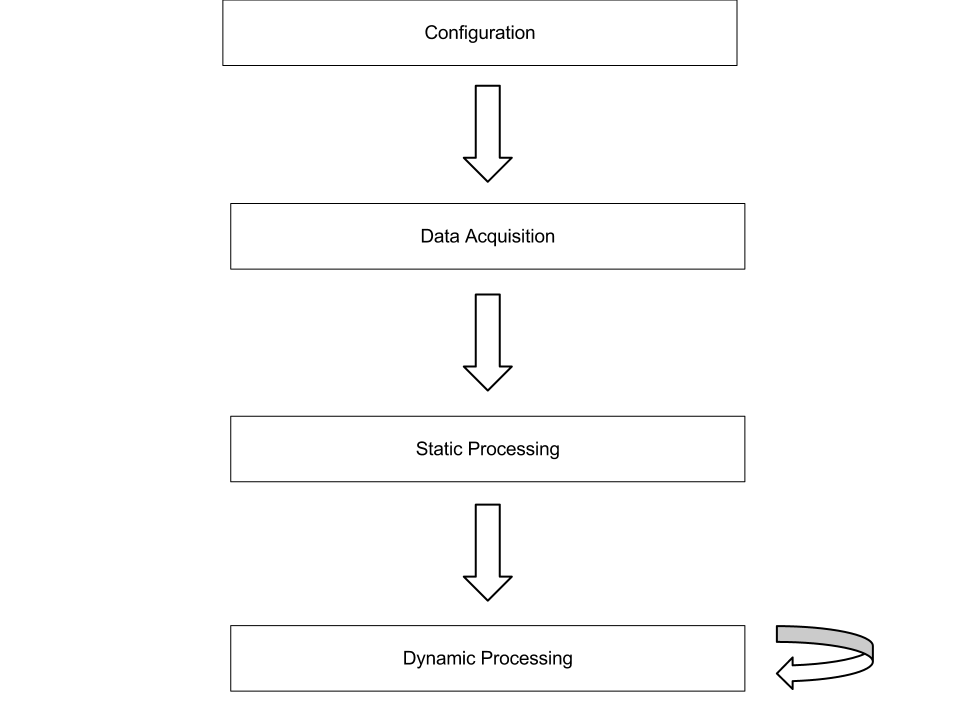
\includegraphics[width=0.45\textwidth]{fig1.png}
\end{figure}

\subsection{Implementation}
The implementation of these blocks is done using two primary languages (C++ and Python) and a host of libraries and modules. As of now, the bulk
of the effort is in C++. Hopefully, applications will reuse the C++ codebase, while the Python toolkit expands for new applications.

\subsubsection{C++}
The configuration, data acquisition, and static processing stages are all accomplished using C++. Configuration uses libconfig, which 
has it's own syntax for configuration files. These configurations files are read in when a program begins in order to configure blocks and 
components. Data acquisition currently has two options: WAV file input and mp3 encoded file input. Depending on the extension of the named file, 
data is stripped using libmpg123 ifor mp3s, or libsndfile for WAV format. Eventually, the data acquisition stage will also include the ability to processes streams of data, as well as CSV and raw binary files. Once the initial timeseries data is obtained, it is loaded into a block which will travel through the entire processing chain, gaining new entries as the data is transformed end manipulated. 

Next, static processing is applied to the data, using compiled blocks of processing code. Currently, the static blocks available perform FFTs, 
Cepstral Transforms, Bark Frequency Cepstral Coefficients, and DCTs. These blocks use libfftw3 and the Eigen template library to perform 
fourier transforms and matrix operations. Once the static processing chain has completed, the data and it's tranform representations are 
loaded into a Python interpreter, which then exposes the computed arrays directly to a configured list of Python scripts to be executed in the dynamic
stage.

\subsubsection{Python}
The Python sections allow a high-level, interactive interface to the data and it's representative transforms. Often, advanced statistical modeling, 
plotting routines, and complex analysis are performed in this stage. Most of these operations take advantage of the wide variety of scientific 
and mathematical packages available for Python. There are also configurable options to run the dynamic stage repeatedly, which allows developers to change the Python scripts and immediately see the results of these changes, without having to redo the expensive data transform computations.

\subsubsection{Diagram}
The system specification shown in Figure 1 can now be represented with implemenation boundaries, as in Figure 2.
\begin{figure}[h!]
\centering
  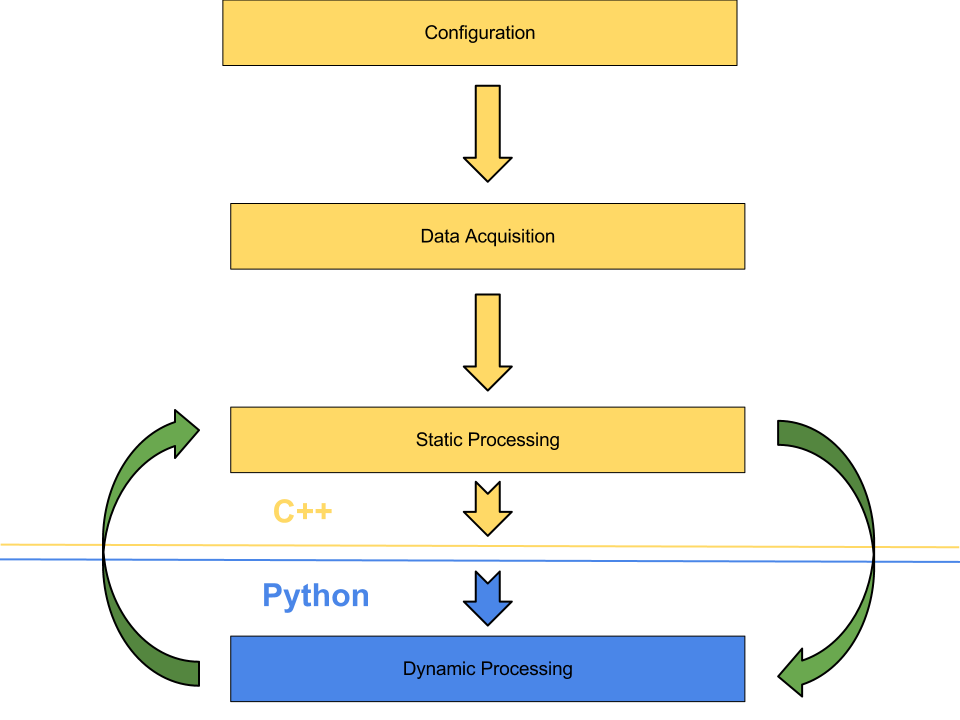
\includegraphics[width=0.45\textwidth]{fig2.png}
\end{figure}

\subsection{Processing}
\subsubsection{Optional File Decompression}
Subsection text here.
\subsubsection{FFT and Power Density}
Subsection text here.
\subsubsection{Cepstrum}
Subsection text here
\subsubsection{DCT}
Subsection text here.
\subsubsection{Bark Filter Bank}
Subsection text here.
\subsubsection{Gaussian Mixture Modeling}
Subsection text here.

\section{Applications}
Subsection text here.

\section{Future Work}
Subsection text here.

\section{Conclusion}
The conclusion goes here.

% if have a single appendix:
%\appendix[Proof of the Zonklar Equations]
% or
%\appendix  % for no appendix heading
% do not use \section anymore after \appendix, only \section*
% is possibly needed

% use appendices with more than one appendix
% then use \section to start each appendix
% you must declare a \section before using any
% \subsection or using \label (\appendices by itself
% starts a section numbered zero.)
%

\appendices
\section{Proof of the First Zonklar Equation}
Appendix one text goes here.

% you can choose not to have a title for an appendix
% if you want by leaving the argument blank
\section{Continued Proof}
Appendix two text goes here.

\begin{thebibliography}{1}

\bibitem{IEEEhowto:kopka}
H.~Kopka and P.~W. Daly, \emph{A Guide to \LaTeX}, 3rd~ed.\hskip 1em plus
  0.5em minus 0.4em\relax Harlow, England: Addison-Wesley, 1999.

\end{thebibliography}

% if you will not have a photo at all:
\begin{IEEEbiographynophoto}{Kyle Kastner}
Kyle Kastner works at Southwest Research Institute, Division 16.
\end{IEEEbiographynophoto}

\begin{IEEEbiographynophoto}{Johanna Hansen}
Johanna Hansen works at Southwest Research Institute, Division 16.
\end{IEEEbiographynophoto}

% You can push biographies down or up by placing
% a \vfill before or after them. The appropriate
% use of \vfill depends on what kind of text is
% on the last page and whether or not the columns
% are being equalized.

%\vfill

% Can be used to pull up biographies so that the bottom of the last one
% is flush with the other column.
%\enlargethispage{-5in}

% that's all folks
\end{document}


